% Please give the surname of the lead author for the running footer
\leadauthor{Tosheva \& Laine}

% info about NM-BC format: https://www.nature.com/nmeth/about/content

\title{NanoJ: a high-performance open-source super-resolution microscopy toolbox}
%NM-BC: The title is limited to 10 words (or 90 characters)
\shorttitle{NanoJ}

% Use letters for affiliations, numbers to show equal authorship (if applicable) and to indicate the corresponding author
\author[1,2\space *]{Kalina L. Tosheva}
\author[1-3\space *]{Romain F. Laine}
%\author[1,2,4]{Nils Gustafsson}
\author[1,2,4]{Robert D. M. Gray}
\author[1,2]{Pedro Almada}
\author[1]{David Albrecht}
\author[1,6]{Tarrason Risa, Gabriel}
\author[7]{Ann-Christin Lindås}
\author[1,6]{Buzz Baum}
\author[1]{Jason Mercer}
\author[5]{Christophe Leterrier}
\author[1-3\space\Letter]{Pedro M. Pereira}
\author[1-3\space\Letter]{Si\^{a}n Culley}
\author[1-3\space\Letter]{Ricardo Henriques}

\affil[1]{MRC-Laboratory for Molecular Cell Biology. University College London, London, UK}
\affil[2]{Department of Cell and Developmental Biology, University College London, London, UK}
\affil[3]{The Francis Crick Institute, London, UK}
\affil[4]{Centre for Mathematics and Physics in Life Sciences and Experimental Biology (CoMPLEX), University College London, London, UK}
\affil[5]{Aix Marseille Université, CNRS, INP UMR7051, Marseille, France}
\affil[6]{Institute for the Physics of Living Systems, University College London, London, UK}
\affil[7]{Department of Molecular Biosciences, The Wenner-Gren Institute, Stockholm University, Stockholm, Sweden}

\affil[*]{These authors contributed equally.}

\maketitle

%TC:break Abstract
\begin{abstract}
%Lets try to keep the abstract between 70-150 words, I have noticed no guidance

Super-Resolution Microscopy has become essential for the study of many nanoscale biological processes. The field generally relies on specialised image analysis tools to routinely process the large volumes of recorded data and robustly extract underlying quantitative information. In recent years, our team has built an image analysis framework for Super-Resolution Microscopy which combines high-performance, open-source and ease of use, which we called NanoJ - a reference to the popular ImageJ software it was developed for. In this paper, we highlight the current capabilities of NanoJ for use in several essential steps of microscopy studies: spatial alignment of the raw data (NanoJ-Core), Super-Resolution image reconstruction (NanoJ-SRRF), image quality assessment (NanoJ-SQUIRREL), structural modelling (NanoJ-VirusMapper) and control of the sample environment (NanoJ-Fluidics). We are constantly expanding NanoJ with the aim to improve quantitative analysis and reliability of biomedical microscopy studies .

\end {abstract}
%TC:break main
%the command above serves to have a word count for the abstract

\begin{keywords}
    ImageJ | Fiji | Super-Resolution Microscopy | Image Analysis | Fluidics | Resolution | Quantitative imaging
\end{keywords}

\begin{corrauthor}
    p.pereira\at ucl.ac.uk, s.culley\at ucl.ac.uk, r.henriques\at ucl.ac.uk
\end{corrauthor}

%%%%%%%%%%%%%%%%
% Introduction %
%%%%%%%%%%%%%%%%
% ------------------------------------------------------------------------------------------------------------------------------------

\subsection*{Introduction}
 Fluorescence microscopy has been ubiquitously used in biological studies since its invention in the 20\textsuperscript{th} century. It underpins most research aiming at observing structures and interactions between specifically labelled molecules, allowing the quantification of their dynamic behaviour in living cells. In recent years, Super-Resolution Microscopy (SRM) \cite{betzig2006imaging,rust2006sub,hell1994breaking} emerged from decades of imaging studies at the single-molecule level and has dramatically expanded the toolbox of fluorescence microscopy. However, extracting biologically relevant quantitative information from any type of fluorescence microscopy data typically requires specialised digital processing and analysis \cite{wheeler2017standard}. Additionally, the increasing amount of data generated by SRM, highlights the need for high-performance image analysis packages.  Several great SRM image processing packages are available such as ThunderSTORM \cite{ovesny2014thunderstorm}, LAMA \cite{Malkusch2016LAMA} or SIMcheck \cite{schermelleh2015simcheck} but each of these are focused on a specific type of SRM modality.
  
 %TC:ignore
 \begin{figure}[!t]
    \centering
    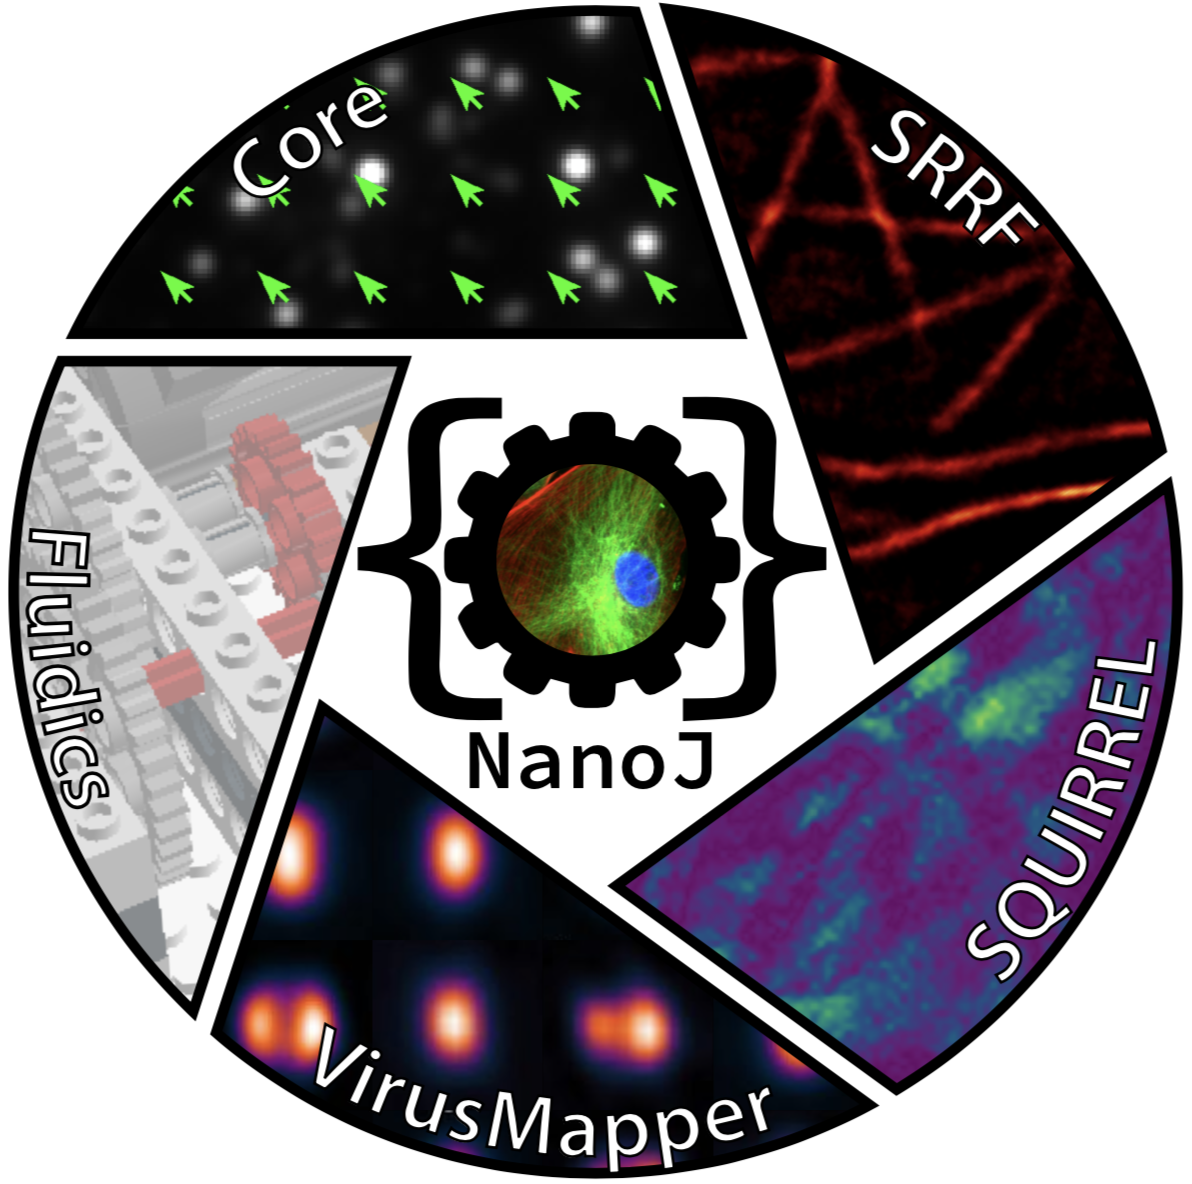
\includegraphics[width=\linewidth]{Figures/Figure1_v3.png}
    \caption{\textbf{NanoJ framework.} Currently NanoJ consists of 5 modules dedicated to enable super-resolution imaging and analysis.}
    \label{fig:GeneralDiagram}
 \end{figure}
 %TC:endignore
  
 Here, we present NanoJ, a highly versatile set of image analysis and acquisition methods developed to aid researchers at many stages of microscopy studies, with a particular focus on the demands of live-cell SRM. NanoJ is available as a series of ImageJ-based plugins which can be used independently or concomitantly to obtain high-fidelity images from which qualitative and quantitative information can be extracted. NanoJ is comprised of (see Fig. \ref{fig:GeneralDiagram}): \textbf{NanoJ-Core} - a set of general image correction tools, which include drift correction and channel realignment, both based on cross-correlation analysis; \textbf{NanoJ-SRRF} - an analytical approach capable of extracting super-resolution data from a short burst sequence of images and that can be acquired with most microscopes \cite{gustafsson2016fast,culley2018srrf}; \textbf{NanoJ-SQUIRREL} - an algorithm to evaluate resolution and the presence of artefacts in super-resolution images \cite{culley2018quantitative}; \textbf{NanoJ-VirusMapper} - a Single-Particle Analysis method to generate nanoscale models of repetitive meta-stable biological structures such as viruses \cite{Gray2016,Gray2017,gray2018nanoscale}; \textbf{NanoJ-Fluidics} - a software interface to control fluidic hardware devices, enabling automation e.g. of multiplexing experiments \cite{almada2018automating}. While these methods were originally developed to address specific biological questions, NanoJ is aimed at solving common imaging problems with broad applications and, thus, is compatible with a multitude of fluorescence microscope setups and experimental protocols. 
 
\subsection*{The NanoJ framework}
 NanoJ has been designed to integrate with the popular ImageJ or Fiji image analysis software \cite{abramoff2004image,schindelin2012fiji}, being easily installed as a standard set of plugins. NanoJ is fully open-source and user-friendly, making use of state-of-the-art algorithms and code execution strategies. The graphical user interfaces (GUIs) are designed to be straightforward to use and its routines can be easily integrated within larger image analysis pipelines through the ImageJ macro language.

 It is broken down as individual modules with corresponding user manuals making it an accessible tool for both non-expert users, as well as developers. It is developed in both Java (\href{https://www.java.com/}{https://www.java.com/}) and OpenCL (\href{https://www.khronos.org/opencl}{https://www.khronos.org/opencl}), the latter language being used for high-performance analysis of image data through the use of Graphical Processing Units (GPUs). As of date, it encompasses four Java ARchive (JAR) packages - NanoJ-SRRF, NanoJ-SQUIRREL, NanoJ-VirusMapper, NanoJ-Fluidics - that all depend on a central package - NanoJ-Core - which contains the libraries that enable high-performance GPU-based computing analysis and a large set of basic image analysis helper methods. The modular nature of NanoJ means that its components can be updated independently and the framework can be easily extended by appending new analytic packages. Furthermore, as part of the NanoJ-Core module, we make a number of benchmarking routines available, capable of exploring the image analysis capabilities (in particular via GPU processing) of the machine used.

\subsection*{NanoJ-Core: Drift Correction}
 During the acquisition of a SRM data there is often a need for the sample to remain static in order to minimise motion blur artefacts and therefore loss of resolution. However, drift commonly occurs in microscopes during acquisition times, often as a result of gradual changes in temperature of system components. While most modern microscopes have an active focus-lock device that stabilises the motion of the sample in the axial direction (minimizing focal drift), the sample will still be prone to lateral movement. However, in the case where the raw data is made up of a sequence of consecutive frames acquired rapidly, as is common in SRM methods such as Single Molecule Localization Microscopy (SMLM) \cite{betzig2006imaging,rust2006sub} or fluctuation-based approaches \cite{gustafsson2016fast,dertinger2009fast,cox2012bayesian}, this lateral drift can be estimated and analytically corrected via post-processing.
 
  %TC:ignore
 \begin{figure}[!t]
    \centering
    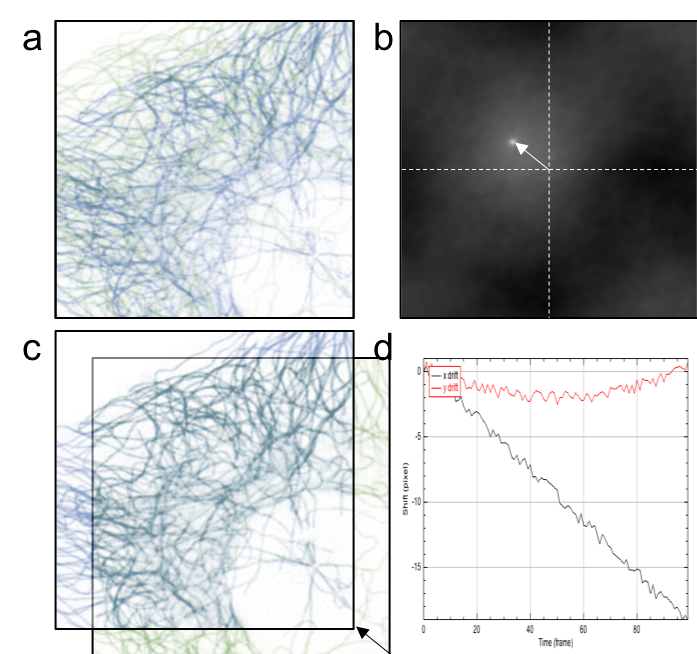
\includegraphics[width=\linewidth]{Figures/Fig2_Drift_Initial.png}
    \caption{\textbf{Drift correction with NanoJ-Core.} \textbf{a)} Composite image of two frames of the same field-of-view with visible drift. \textbf{b)} Cross-correlation map between the two frames shown in a). The vector position of the maximum indicates the linear shift between the two frames. \textbf{c)} Overlay of the two frames after drift correction using NanoJ-Core. \textbf{d)} Example vertical and horizontal drift curves obtained from 100 consecutive frames.}
    \label{fig:DriftCorrection}
 \end{figure}
 %TC:endignore

 NanoJ breaks the task of drift correction into the distinct parts of estimation and then translation. NanoJ-Core estimates the linear drift between two images by calculating their cross-correlation matrix (CCM) (see Fig.\ref{fig:DriftCorrection}). The location of the peak intensity in the CCM determines the linear shift between the two images and here is precisely estimated by up-scaling the CCM, using a bicubic-spline interpolation, thus achieving sub-pixel accuracy. Depending on the type of acquisition, the reference frame can either be the first frame of the raw data (for a fixed sample for instance) or the preceding SRM frame (for a live sample). Fig. \ref{fig:DriftCorrection}d shows how the drift with respect to the first frames can be followed in time in a representative 100 frames dataset, and therefore corrected. Once drift is estimated, the dataset can be directly corrected by analytically translating each individual frame using a bicubic-spline interpolation. The interpolation process will however change the noise properties of the resulting dataset \cite{blaysat2016effect}.
 
 For the specific case of SMLM datasets with sparse blinking, there will only be a weak correlation across frames, as there is little observable structure conserved between time points. One common strategy to alleviate this low correlation is to add fiduciary landmarks to the sample, such as static fluorescent beads. NanoJ-Core offers an alternative to the use of fiducial markers by temporally binning the dataset, thus increasing the correlation between binned frames and allowing their shift to be precisely estimated \cite{mlodzianoski2011sample}. 

 Drift estimation in NanoJ therefore differentiates from other strategies applied by other SRM algorithms, such as ThunderSTORM \cite{ovesny2014thunderstorm}, by the fact that it analyses originally acquired unprocessed data, instead of post-processed Super-Resolution reconstructions. This allows the estimation to be decoupled from the Super-Resolution analysis strategy used, thus enabling further methods such as SRRF or SOFI \cite{dertinger2009fast} to benefit from it. Alternatively, algorithms such as NanoJ-SRRF can import the created drift-table, directly using this information during analysis without the need to pre-translate each frame in the raw dataset.

\subsection*{NanoJ-Core: Channel Alignment}

 Images captured with a fluorescence microscope in different spectral channels often appear misaligned, as a result of chromatic aberrations in the optical systems and from using different spectral filters between the channels. While in conventional microscopy both of these effects can often be ignored, provided they occur at a scale smaller than the diffraction limit, their effect can become substantial in the context of SRM. This leads to an increasingly perceivable discrepancy between spatial structures observed in different spectral channels as resolution increases \cite{erdelyi2013correcting}. It is therefore essential to correct this spectral misalignment in multi-colour SRM studies, especially when it involves the quantification of colocalisation between different structures \cite{bock2007two,van2009multicolor,niekamp2017high}. 
 
 The shift between different spectral channels often varies non-linearly with the position across the image, which prevents using typical CCM-based approaches, such as the one used by NanoJ-Core Drift Correction. A common approach to estimate the shift is to image a sample showing the same structure across all the relevant wavelength channels, where this structure occupies a large portion of the imaged field-of-view, e.g. a coverslip with a high-density of randomly placed multi-spectral beads. This dataset can be used to extract a non-linear spatial transform for each spectral channel with respect to a reference channel, and these transforms can then be used to re-align all further multi-spectral dataset \cite{arganda2006consistent,annibale2012identification}. 
 
 Because the correction necessary here is spatially varying across the image (see Fig.\ref{fig:ChannelAlignment}a), NanoJ takes the approach of breaking the image down into small areas, which are in turn compared to the equivalent area in the reference channel. Locally, the correction can be assumed to be linear and the linear shift can be estimated by finding the cross-correlation peak position as shown in Fig.\ref{fig:DriftCorrection}ab. An inverse distance weighting interpolation \cite{shepard1968two} is used to smoothly determine shift values across the whole field-of-view, including the areas that do not contain any structure in the calibration dataset. This approach allows us to extract a shift map (in both vertical and horizontal directions) that can be applied to further datasets (see Fig.\ref{fig:ChannelAlignment}b). The amplitude of the horizontal and vertical shift maps represent the physical shift associated with each direction and that needs be to locally to re-align the corresponding channel to the reference channel. These shift maps have the benefit of easily highlighting the chromatic distortion across the field-of-view, helping with the assessment of the image quality. 
 
 \begin{figure}[!t]
    \centering
    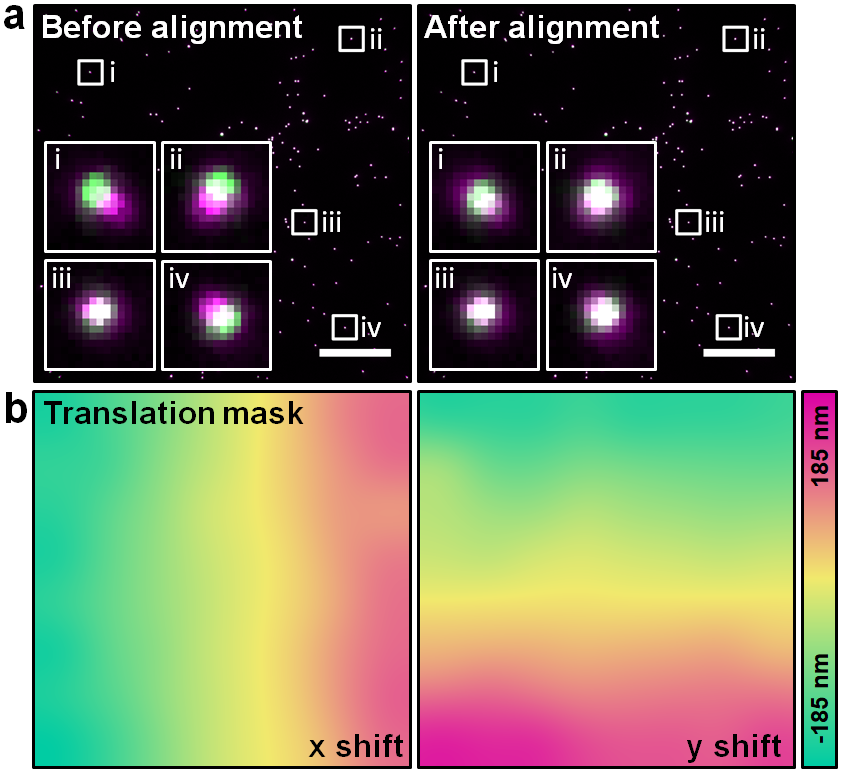
\includegraphics[width=\linewidth]{Figures/Test_Figure_3.png}
    \caption{\textbf{Multi-colour channel alignment with NanoJ-Core.} \textbf{a)} Composite image of multi-colour TetraSpeck beads imaged in two different channels (GFP channel indicated in green and mCherry channel in magenta), prior to (left) and after (right) channel re-alignment using NanoJ-Core, acquired on a Nikon Ti2 frame with the CFI Apochromat TIRF 100XC Oil objective. Insets - individual beads from indicated locations, 1.63 x 1.63 \micro m. Scale bars: 25 \micro m. \textbf{b)} Horizontal and vertical shift maps obtaiend and applied to the data shown in a). Scale bars: 25 \micro m.}
    \label{fig:ChannelAlignment}
\end{figure}
 
 The channel alignment correction is then achieved on any multi-color dataset by creating a new image representing each channel, where the intensity value for each pixel coordinate corresponds to the intensity value from the original image at the equivalent coordinate corrected for local shift. For the cases where these coordinates are not discrete (sub-pixel shift), a bicubic-spline interpolation is used to recover pixel values in continuous space. Because the shift map can be extrapolated to continuous space, the alignment procedure obtained from diffraction-limited images can also easily be used to correct SRM dataset of any resolution. 
 
\subsection*{NanoJ-SRRF: Live-Cell Super-Resolution Imaging}
 As part of the NanoJ framework, we include our recently developed SRM reconstruction algorithm called Super-Resolution Radial Fluctuations (SRRF), able to extract sub-diffraction information from a short burst of images acquired at high-speed with modern fluorescence microscopes \cite{gustafsson2016fast,culley2018srrf}. SRRF is a purely analytical approach and, compared to other SRM methods, it alleviates the need to use toxic photoswitching-inducing buffers \cite{henriques2011palm}, specialised fluorophores \cite{dempsey2011evaluation,henriques2009palm}, damaging high-intensity illumination \cite{waldchen2015light} or specialised equipment \cite{gustafsson2000surpassing,hell1994breaking}.
 
 %TC:ignore
\begin{figure}[!t]
    \centering
    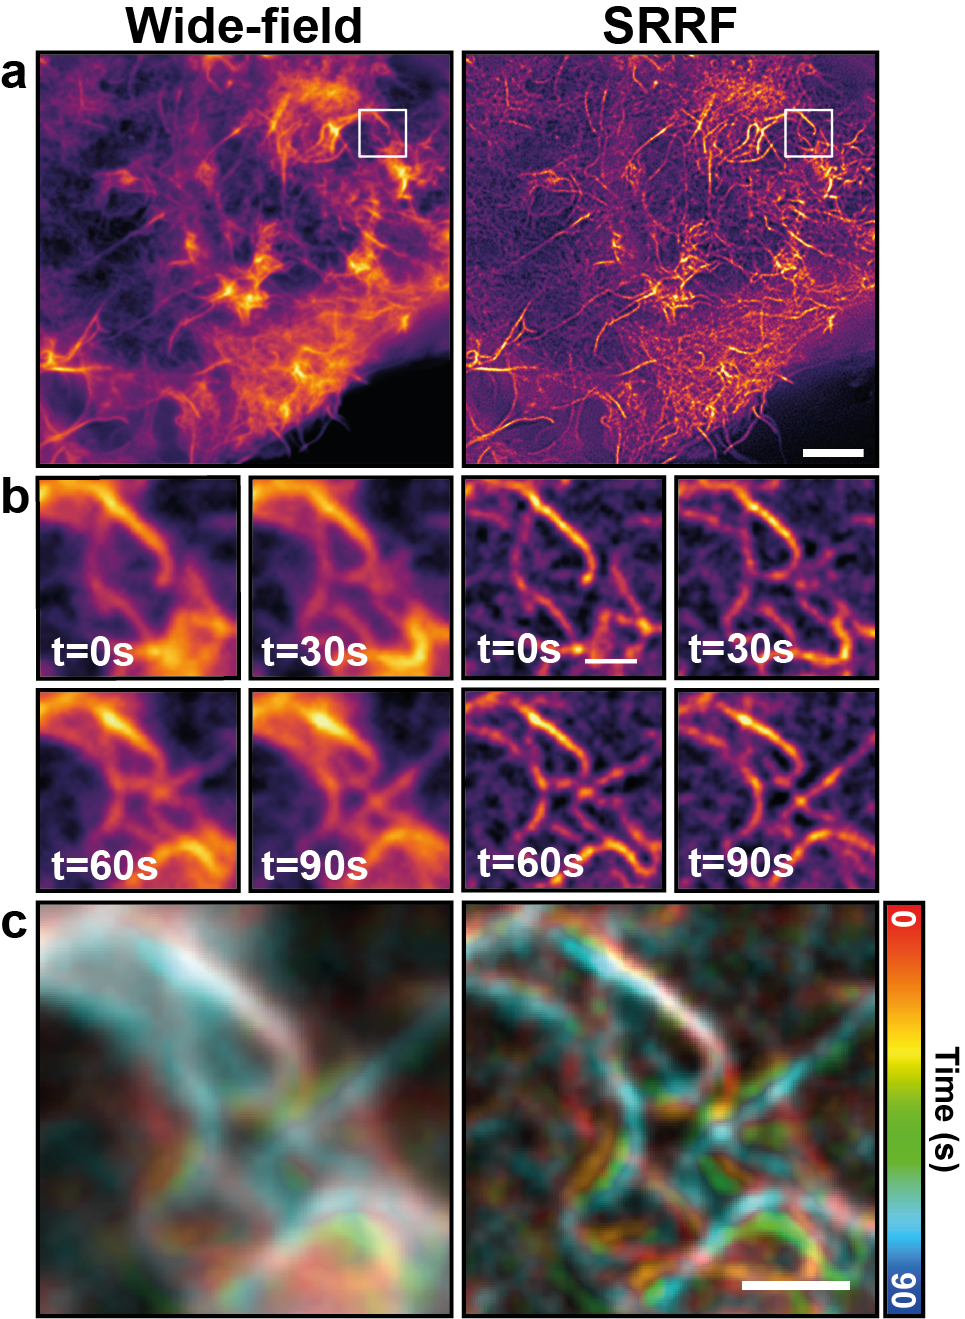
\includegraphics[width=\linewidth]{Figures/Figure4_v3.png}
    \caption{\textbf{Live-cell super-resolution with NanoJ-SRRF.} \textbf{a)} Comparison of wide-field (left) and SRRF reconstruction (right) obtained from a Cos7 cell expressing UtrCH-GFP. Scale bar: 5 \micro m. \textbf{b)} Time-course of the inset shown in a), obtained from  a continuous imaging at 30 ms exposure (33.3 Hz) and displayed every 30 s. Scale bar: 1 \micro m. \textbf{c)} Colour-coded time course dataset from b). Scale bar: 1 \micro m.}
    \label{fig:SRRF}
\end{figure}
%TC:endignore
 
 SRRF is based on similar principles to SMLM, however it does not rely on the detection of spatio-temporally isolated fluorophore. In comparison, SRRF generates a magnified pixel grid where each pixel value relates to the probability of fluorophores existing in that corresponding region of space. To do so, SRRF calculates the local radial symmetry in each sub-pixel of the magnified image using local intensity gradient information. The obtained radiality transform will be high when a point-spread-function (PSF) profile transiently becomes dominant, highlighting the presence of a fluorescent molecules in that location. Also, the fluctuation of local radiality follows the underlying natural intensity fluctuation of fluorophores, which has a distinct temporal signature to that of noise \cite{dertinger2009fast}. A temporal correlation of radial symmetries at each pixel can then be projected into a final image, where the structures of interest can be better resolved (see Fig.\ref{fig:SRRF}a).
 
 Practically, a typical SRRF image is generated by analysing $\sim$100 frames imaged at 100Hz, using an acquired image pixel size of $\sim$100nm. These values are generally a good estimate to achieve a high-quality SRRF image, but should however be optimised for each sample, in order to improve both image quality and resolution. Optimally, the pixel size should match the Nyquist criterion for the objective and wavelength detected \cite{pawley2010handbook}, the frame-rate needs to be sufficiently high to temporally sample fluorophore oscillations, and the number of frames collected sufficient for SRRF to accurately represent structure distinct from noise. SRRF is highly compatible with live-cell SRM and allows long time-course acquisition. Fig.\ref{fig:SRRF}b and c show a typical live-cell SRRF acquisition of a Cos7 cell expressing UtrCH-GFP (actin marker) imaged at 33.3 Hz for > 30 min with no visible phototoxicity. Here, SRRF allows a detailed observation of actin dynamics at super-resolution.
 
 NanoJ-SRRF, the software implementation of the SRRF algorithm, uses whenever possible GPU high-performance computing to accelerate the radial symmetry estimation. This is achieved by implementing a large set of the needed SRRF calculations in OpenCL, with a fallback of execution to the CPU using standard Java when a compatible graphics card is not found. NanoJ-SRRF can use a drift-table as an additional input, dynamically using its values to compensate for unwanted sample drift during the calculation of radial symmetries and temporal correlations.

\subsection*{NanoJ-SQUIRREL: Estimating Image Quality}
All SRM techniques require additional complexity compared to conventional diffraction-limited microscopy. This complexity arises from the sample preparation (SMLM), the microscope hardware (STED, SIM) and the post-acquisition image processing (SMLM, SIM). Inappropriate choices of these acquisition and reconstruction parameters can lead to artefacts within the final image and the potential for false conclusions to be drawn. NanoJ-SQUIRREL (Super-resolution Quantitative Image Rating and Reporting of Error Locations) is an algorithm that highlights the presence of artefacts and can thus be used to assess super-resolution image quality and optimise acquisition pipelines.

The central concept of SQUIRREL is that a diffraction-limited image and the corresponding super-resolution rendering of the same region should relate to the same underlying structure, just at different resolutions. This concept implies that it is possible to simply blur the SRM image decrease its resolution to achieve an equivalent diffraction-limited image. Any discrepancy between true diffraction limited and the blurred SRM will therefore originate from artefacts and non-linearity in the reconstruction and imaging.

NanoJ-SQUIRREL analytically formalises this notion by estimating the blurring function to apply to the SRM image and computing an error map, representing the difference between the true diffraction-limited and the blurred SRM image. Two global quality metrics are also generated: the RSP (Resolution Scaled Pearson’s Correlation Coefficient) and the RSE (Resolution Scaled Error). The RSP can take a value in the interval [-1,1] and describes the structural agreement between the super-resolution and reference images. Here, higher values indicate better agreement, with an RSP of 1 indicating a perfect structural match. The RSE describes the sum intensity mismatch between the super-resolution and reference images; in this case lower values represent better agreement with a value of 0 indicating a perfect intensity match. Fig.\ref{fig:SQUIRREL}a and b shows super-resolution image, its corresponding diffraction-limited (widefield) image and the error map obtained from NanoJ0-SQUIRREL. The three insets shown in Fig.\ref{fig:SQUIRREL}b indicate areas where typical STORM artefact are present to different extent (mislocalization, bridging artefacts or missing localisation \cite{waldchen2015light}). 

% Quality assessment in SQUIRREL requires the user to provide a diffraction-limited `reference’ image and super-resolution rendering of the same structure. If both images accurately represent the underlying fluorophore distribution but at different resolutions then there exists a blurring, or `resolution scaling’, function that can convert a super-resolution image into its diffraction-limited equivalent. SQUIRREL calculates this resolution scaling function and applies it to the super-resolution image, and the blurred super-resolution image is then compared against the reference image. During this comparison, three quality indicators are generated. An `error map’ is produced that maps the discrepancy between the blurred super-resolution image and the reference image at every pixel. This highlights local regions where the super-resolution image is inconsistent with the reference image. 


%TC:ignore
\begin{figure}[!t]
    \centering
    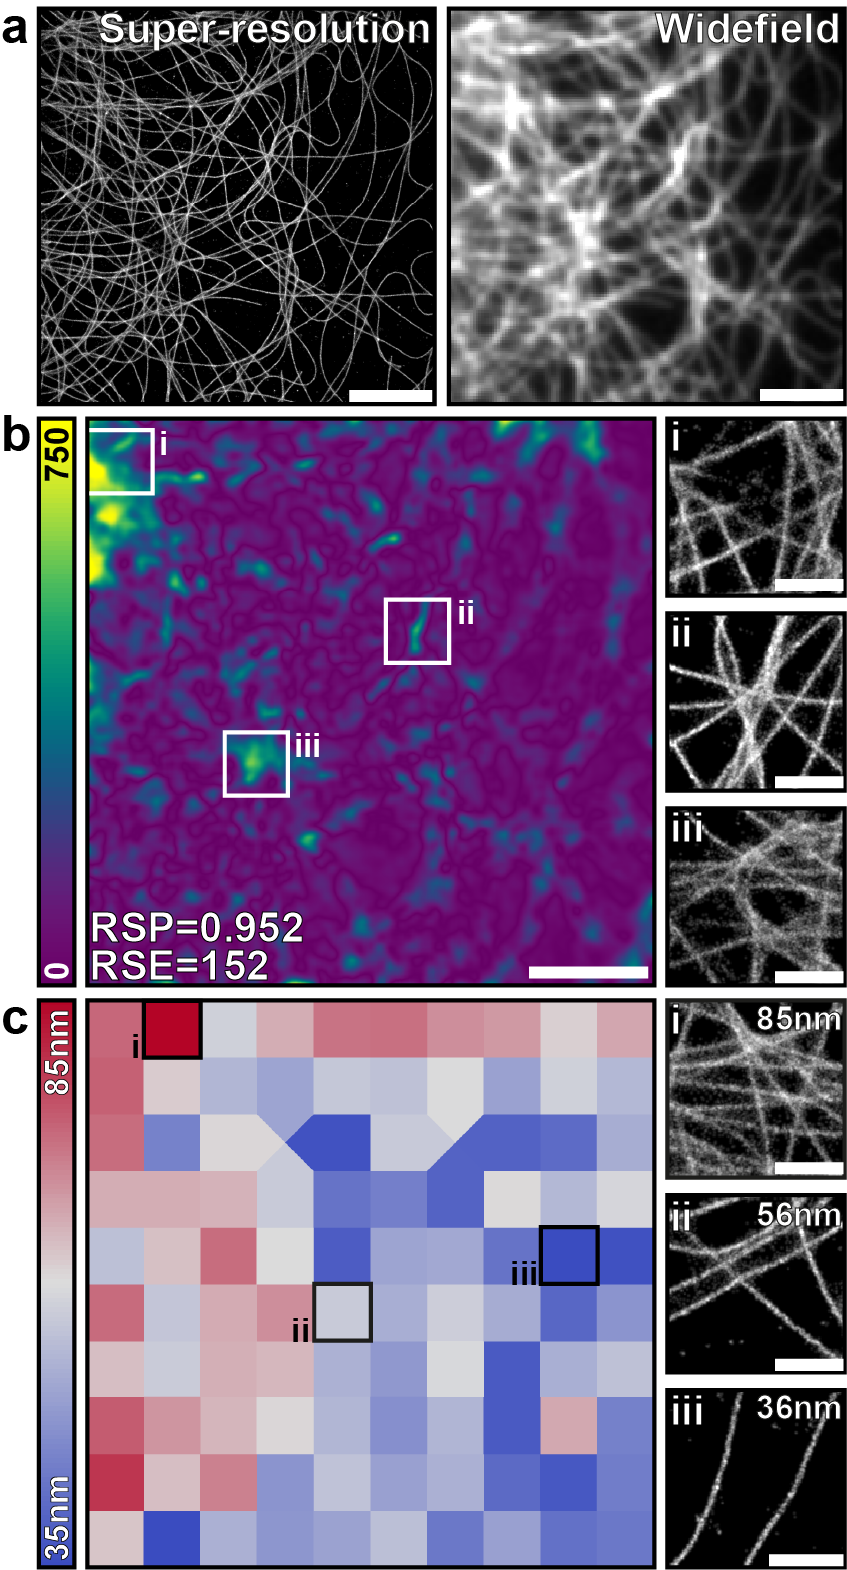
\includegraphics[width=\linewidth]{Figures/SQUIRREL_draft_column_format.png}
    \caption{\textbf{Quality assessment and resolution mapping with NanoJ-SQUIRREL.} \textbf{a)} A super-resolution rendering (left) and acquired widefield image (right) of fixed microtubules labelled with Alexa Fluor-647. \textbf{b)} Left: SQUIRREL error map highlighting discrepancies between the super-resolution and diffraction-limited images in (a). Right: Magnified insets of super-resolution rendering at indicated positions on error map. \textbf{c)} Left: SQUIRREL resolution map of the super-resolution image in (a). Right: Magnified insets of super-resolution rendering for indicated resolution blocks. Whole image scale bars = 5\micro m, inset scale bars = 1\micro m}
    \label{fig:SQUIRREL}
\end{figure}
%TC:endignore

\subsection*{NanoJ-SQUIRREL: Estimating Image Resolution}
The purpose of SRM is to resolve finer structural detail than is achievable with conventional diffraction-limited microscopy. It is therefore useful to have an objective measurement of spatial resolution within a super-resolution image to enable comparisons with known structure sizes from electron microscopy and for performance assessment of newly developed super-resolution techniques. The current standard for estimating image resolution in SRM images is Fourier Ring Correlation (FRC, \cite{nieuwenhuizen2013measuring}). This method involves comparing two super-resolution images of the same field-of-view so that they only differ by their noise component. For example, for SMLM datasets, the two SRM images can be obtained by splitting localisations from odd and even frames. The correlation between these two images is measured at different frequencies in Fourier space; the frequency at which this correlation drops below a set threshold indicates the resolution of the image.

FRC has been previously implemented in ImageJ \cite{nieuwenhuizen2013measuring}, but only gives a single resolution measurement for the entire field of view. However, resolution is not necessarily homogeneous across a super-resolution image. This is particularly true for SMLM methods as localisation accuracy depends strongly on labelling density and laser illumination intensity, which can both vary considerably within a single field of view. Furthermore, FRC can generate biased measurements for certain fluorophore distributions such as point-like patterns. Therefore an additional feature of the NanoJ-SQUIRREL plugin is local mapping of FRC resolution across an image. To do this, the user provides an image stack comprising two independent renderings of the same dataset (e.g. through the odd/even frames splitting as described above). The images are then split into equally-sized blocks and FRC analysis is run locally on each block. For blocks where there is insufficient correlation to generate an FRC resolution value, a resolution value is interpolated from neighbouring blocks. Fig.\ref{fig:SQUIRREL}c shows the FRC map obtained from a 10x10 blocks of the SRM image shown in (a). This map highlights that the resolution in this image varies between 85 and 36 nm, as highlighted by the insets.

It is important to note that high resolution (that is, a low FRC value) does not imply that the super-resolution image has depicted structures correctly; it only means that there is low variation in the locations of the fluorophores between the two rendered images. Therefore it is advisable to use the error mapping functionality within NanoJ-SQUIRREL alongside FRC mapping in order to obtain a more complete view of super-resolution image quality.


\subsection*{NanoJ-VirusMapper: Structural Mapping and Modelling}
As part of the NanoJ framework, we include a unique single particle analysis (SPA) tool called NanoJ-VirusMapper. It is the first freely available algorithm for unbiased, high-throughput SPA of fluorescence imaging and allows the structural modelling of viruses and other macro-molecular complexes \cite{Gray2016,Gray2017}. The principle of SPA is to image many identical copies of a structure, possibly in different orientation, align and combine them to build a high signal-to-noise map of the underlying structure \cite{Szymborska2013,laine2015structural} . 

The SPA implementation of VirusMapper facilitates automatic processing of multiple images to detect, segment, align, classify and average thousands of individual structures from the dataset. Unlike other applications of the technique it is entirely general, assuming no underlying symmetry or properties of the imaged structure. Here, we illustrate this with models of components of vaccinia virus (REF Fields virology), a large mammalian virus with three distinct substructures: a core, lateral bodies (LBs) and a membrane. Here, all three substructures were labelled on viral particles and  imaged with structured illumination microscopy (SIM) \cite{gustafsson2000surpassing} (see Fig.\ref{fig:VirusMapper}a, top). The SIM images from each channel were then independently processed with VirusMapper to create models of the three components of the virus (see Fig.\ref{fig:VirusMapper}a, bottom). Additionally, a key advantage of VirusMapper is that models from different channels can be aligned to each other.

Also, VirusMapper is capable of identifying and analysing different orientation of the same structure. Here, we highlight this capability on a study of the division ring in the archaea \emph{Sulfolobus} (REF) (see Fig.\ref{fig:VirusMapper}b). \emph{Sulfolobus} cells were labelled for their outer S-layer and the division ring as marked by ESCRT-III proteins. Here, the models from both channels were built from aligning the S-layer channel.

VirusMapper has been demonstrated with SIM and stimulated emission depletetion (STED) microscopy \cite{Gray2016} but is compatible with any fluorescence microscopy method, including SRM.

\begin{figure}[!t]
    \centering
    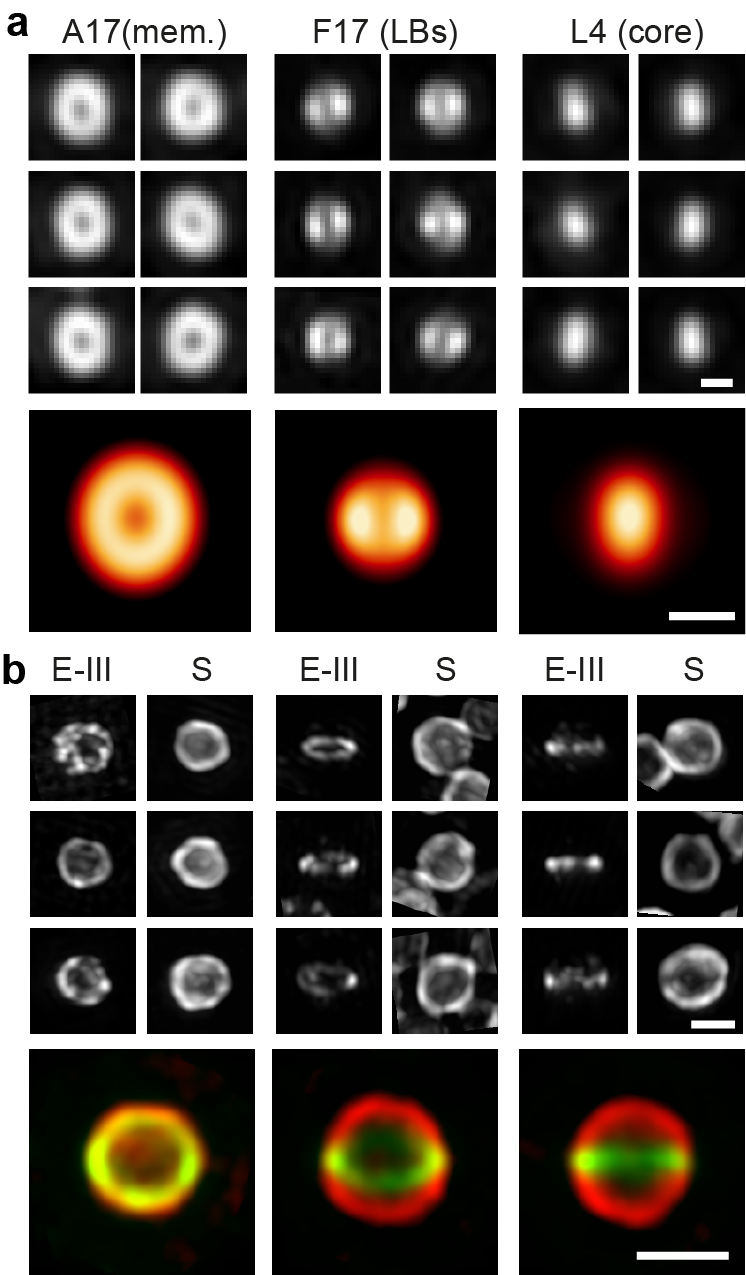
\includegraphics[width=\linewidth]{Figures/NanoJ_VirusMapperFigure_rot.png}
    \caption{\textbf{Quantitative SPA-based modelling with NanoJ-VirusMapper.} \textbf{a)} Top: SIM images of individual vaccinia particles labelled for L4 (core), F17 (lateral body, LB) and A17 (membrane, mem.). Bottom: VirusMapper models of the three channels. Scale bars: 200nm. \textbf{b)} Top: SIM images of individual \emph{Sulfolobus} cells labelled for the S-layer (S) and ESCRT-III (E-III). Bottom: VirusMapper models of three different orientations of the cells. Scale bars: 1\micro m. }
    \label{fig:VirusMapper}
\end{figure}


\subsection*{NanoJ-Fluidics: Sample Liquid Exchange}
%Pereira will write this part
NanoJ-Fluidics is a hardware and software framework for precise and accurate automated fluidics exchange \cite{almada2018automating}. It is developed in order to enable automation of sample treatment and labelling of live or fixed cells directly on the microscope stage. NanoJ-Fluidics hardware is composed of customisable, low-cost and robust LEGO® syringe pumps and a fluid removal peristaltic pump, both controlled by simple Arduino® electronics. It is also compatible with off-the-shelf imaging chambers, without the need for any microfabrication. Its control software is ImageJ-based and can be fully integrated with microscopy acquisition software. We have demonstrated NanoJ-Fluidics applicability in multiple experimental context: \textit{in-situ} correlative live-to-fixed super-resolution imaging, multimodal super-resolution imaging and event-driven fixation \cite{almada2018automating}, but the approach can be easily  extended to protocol optimization (e.g. antibodies concentration or imaging buffer composition) or liquid exchange protocols integrated with the imaging (e.g. drug delivery or automated event-driven fixation).

Here, we present NanoJ-Fluidics on high-quality multicolour SMLM dataset, by combining STORM and DNA-PAINT \cite{jungmann2014multiplexed} into a single NanoJ-Fluidics workflow (see Fig.\ref{fig:PAINT}a). Our approach is perfectly suited to imaging strategies such as the challenging case of multiple labels imaging \cite{dempsey2011evaluation}. With NanoJ-Fluidics we can seamlessly perform all labelling steps in an automated and reliable manner directly on the microscope stage. We showcase this with a 4-channel acquisition of actin with STORM and mitochondria, vimentin and clathrin with DNA-PAINT (Fig. \ref{fig:PAINT}b). 

NanoJ-Fluidics' highly customizable nature has already allowed several alternative designs from the community (\href{https://github.com/HenriquesLab/NanoJ-Fluidics/wiki}{https://github.com/HenriquesLab/NanoJ-Fluidics/wiki}), which are in constant development. NanoJ-Fluidics makes imaging protocol automation available to researchers, this way improving not only the reliability, and repeatability of the protocols but also the scope of protocols that are achievable.  

%TC:ignore
\begin{figure}[!t]
    \centering
    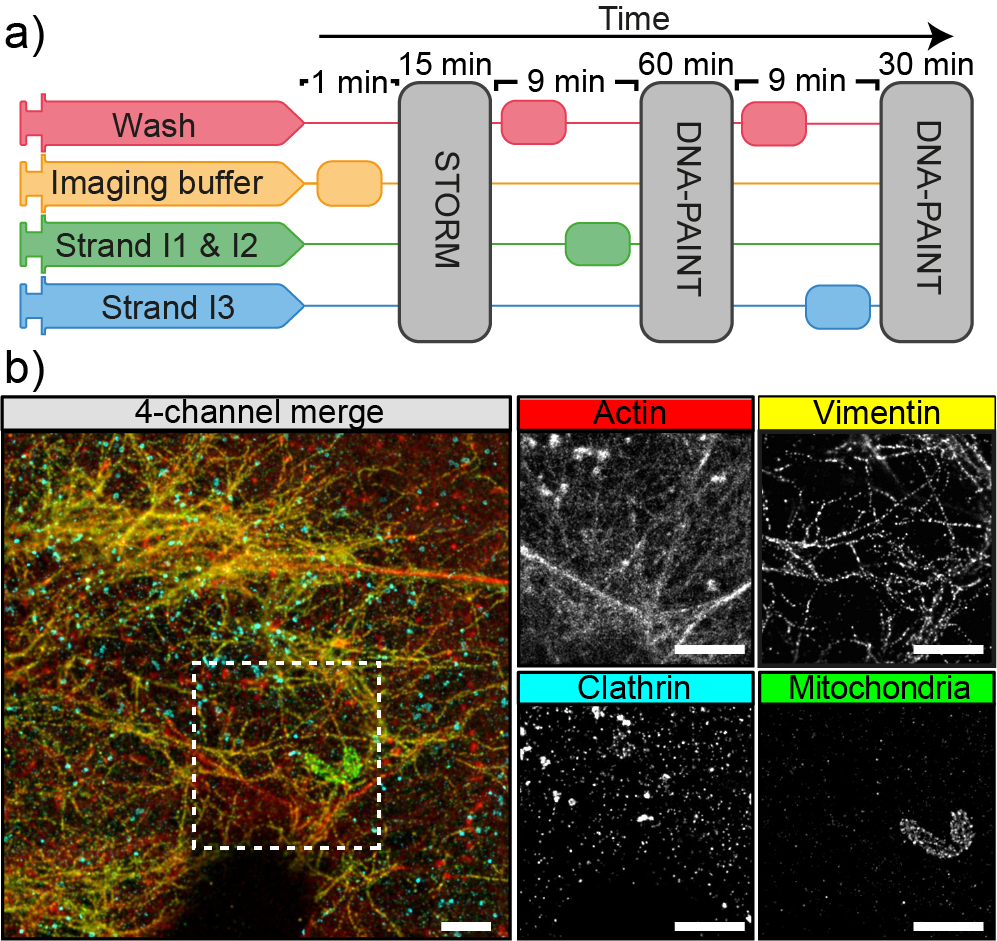
\includegraphics[width=\linewidth]{Figures/Figure5_v2.png}
    \caption{\textbf{Automated DNA-PAINT and STORM imaging.} \textbf{a)} NanoJ-Fluidics workflow used for multi-color STORM and DNA-PAINT imaging. \textbf{b)} 4-channel merge of STORM and DNA-PAINT with actin (red), vimentin (yellow), clathrin (cyan) and mitochondria (green). On the right, Single-channel images from the inset shown on the left. Scale bars: 2 \textmu{}m.}
    \label{fig:PAINT}
\end{figure}
%TC:endignore

\subsection*{Discussion and Future Perspectives}
%KTL, RL and RH will write this part
 The NanoJ framework provides a novel and unique set of comprehensive tools to support biomedical researchers along the experimental pathway, from data acquisition and protocol optimisation down to the structural quantification of image data. It highlights and offers powerful solutions to common pitfalls of image analysis such as drift correction and channel alignment (NanoJ-Core). Our work on developing analytical approach to SRM (NanoJ-SRRF) aligns with the general aim of the community to extend SRM to living cell contexts, which still remains challenging for the common SRM approaches such as STORM and STED. We also place an emphasis on the importance of quantitatively assessing image data quality not only by a single global resolution metrics but also by spatially-varying FRC resolution maps and error (artefacts) mapping (NanoJ-SQUIRREL). Our work in this context aims at objectively exploring the limitations of SRM, and more generally at improving standards in assessing and reporting microscopy studies. In our lab, the workflows of live-cell SRRF imaging studies follow the systematic routine of drift/channel alignment and optimisation of acquisition and reconstruction using SQUIRREL. This ensures that our quantitative analysis are of the best scientific standards.
 
 We are continuously supporting, adapting and expanding the framework to include new approaches. We hope NanoJ can set a standard of useful, open-source, high performance for the whole microscopy community.
 

\subsection*{Software and Hardware Availability}
 NanoJ follows open-source software and hardware standards. Each of its modules can be installed by enabling the corresponding code repository in Fiji or by following the instructions on the corresponding websites:
 \small
 \begin{itemize}
  \item \href{https://github.com/HenriquesLab/NanoJ-Core}{https://github.com/HenriquesLab/NanoJ-Core}
  \item \href{https://github.com/HenriquesLab/NanoJ-SRRF}{https://github.com/HenriquesLab/NanoJ-SRRF}
  \item \href{https://bitbucket.org/rhenriqueslab/nanoj-squirrel}{https://bitbucket.org/rhenriqueslab/NanoJ-SQUIRREL}
  \item \href{https://bitbucket.org/rhenriqueslab/NanoJ-VirusMapper}{https://bitbucket.org/rhenriqueslab/NanoJ-VirusMapper}
  \item \href{https://github.com/HenriquesLab/NanoJ-Fluidics}{https://github.com/HenriquesLab/NanoJ-Fluidics}
\end{itemize}


% \subsection*{Super-Resolution reconstruction}
% % this section is about SRRF, Romain, 500 words max
% As part of our effort to push the limit of live-cell super-resolution microscopy, we developed an analytical approach that allows an increase in resolution without the requirement for toxic buffers  (ref SMLM), damaging high-intensity illumination (ref STED, SMLM) or specialised equipment (SIM, STED ref) from a sufficient number of frames (typically ~100 frames) acquired in a live sample \cite{gustafsson2016fast}. Our method, called SRRF for Super-resolution radial fluctuation, requires  illumination in the and is compatible with all microscopy modality with high resolution \cite{culley2018srrf}. 


% %TC:ignore
% \begin{figure}[!t]
%     \centering
%     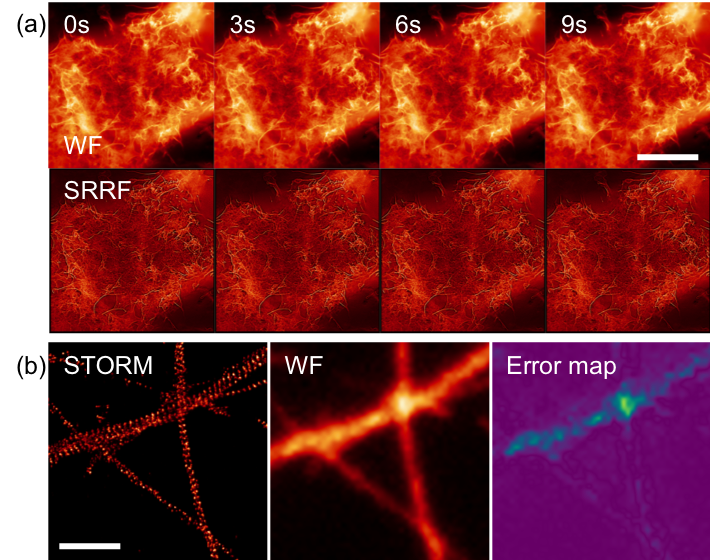
\includegraphics[width=\linewidth]{Figures/Figure4_v1.png}
%     \caption{\textbf{NanoJ - SRRF and SQUIRREL} (a) SRRF analysis on live Cos7 cells expressing UtrCH-GFP imaged every 30 ms and reconstructed every 100 frames (3s time interval between super-resolved images). Scale bar: 20 \textmu{}m. (b) SQUIRREL analysis of STORM imaging of spectrin labelled with AlexaFluor 647 in neurons. Scale bar: 20 \textmu{}m. WF: wide-field.}
%     \label{fig:SRRF&SQUIRREL}
% \end{figure}
% %TC:endignore

% Panel (a) of Figure \ref{fig:SRRF&SQUIRREL} shows the resolution improvement achievable with a typical live-cell experiments, here Cos7 cells with actin labelling. The raw data was acquired with an exposure time of 30 ms and therefore allowed for a temporal resolution of 3s / super-resolved image without any visible phototoxicity or photobleaching to the cell. Yo, can you please fix the contrast for the SRRF images to be the same as for the diff lim ones? Otherwise, to the naked eye, the SRRF ones look uglier...-Kalina


% \subsection*{NanoJ-Fluidics: Sample manipulation during imaging}
% % this section is about pumpy (PMP, ask Christophe if he has another 5 colour pumpy dataset), 500 words max
% We strive to develop the tools necessary for microscopy to be as robust and effective as possible when studying biological systems. This includes developing open-source hardware that is highly enabling for the microscopy community. With this concept in mind, we developed NanoJ-Fluidics (aka "Pumpy McPumpface") \cite{almada2018automating}, an automated fluidics system for \textit{in situ} treatment of the sample. Figure \ref{fig:Pumpy} shows how automated fluid exchange allows the measurement of a 5-color single-molecule localization microscopy (SMLM) of a single fixed cell. Here, a combination of  STORM (Stochastic Optical Reconstruction Microscopy) \cite{rust2006sub, heilemann2008subdiffraction} and DNA-PAINT (DNA- Point Accumulation for Imaging Nanoscale Topography) \cite{sharonov2006wide, jungmann2014multiplexed} modalities was utilised.

% Here, the NanoJ platform integrates the hardware control of the fluidics pumps and interface with  microscopy acquisition through the popular MicroManager platform \cite{edelstein2010computer}. 

% %TC:ignore
% \begin{figure}[!t]
%     \centering
%     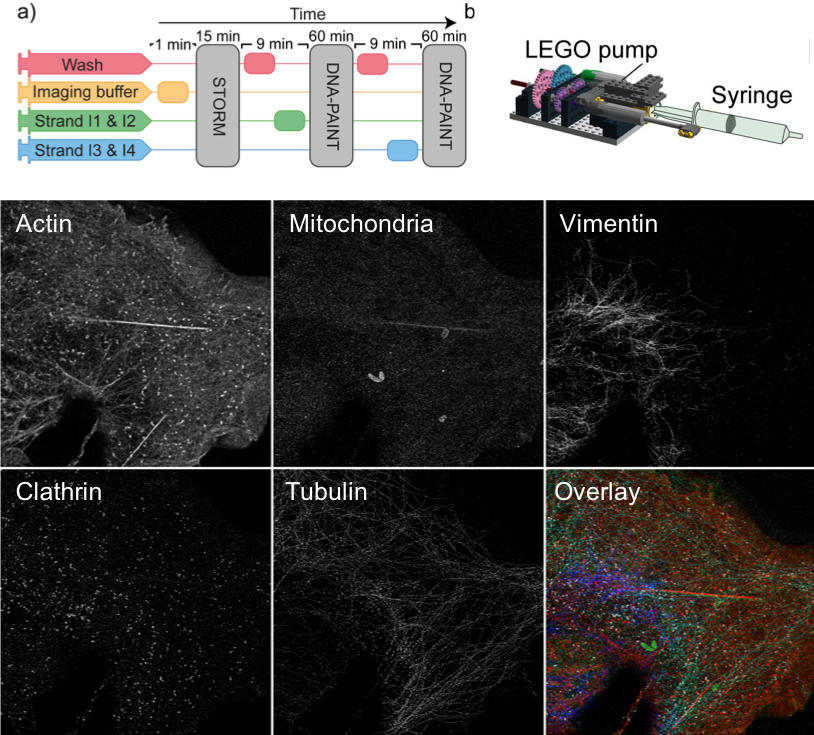
\includegraphics[width=\linewidth]{Figures/Figure2_v2.png}
%     \caption{\textbf{NanoJ-Fluidics} NanoJ-Fluidics allows for automated buffer and sample treatment exchange. (a) Imaging scheme. (b) A single pump from NanoJ-Fluidics. (c) 5-color SMLM imaging obtained on an individual cell.}
%     \label{fig:Pumpy}
% \end{figure}
% %TC:endignore


% \subsection*{Super-Resolution quality control}
% Although super-resolution microscopy has proven to be very powerful in many fields of biology, they are nevertheless prone to artefacts.These artefacts typically come from biases or non-linearities at the stage of image reconstruction. For single-molecule localization microscopy (SMLM) for instance, local high density of emitters can cause bridge artefacts or missing structures \cite{burgert2015artifacts}. In general, all super-resolution microscopy based on analytical approaches suffer from artefacts. We are addressing this issue by developing an algorithm capable of highlighting the presence of artefacts in a super-resolution image by comparing it to its non-super-resolved equivalent. Our method, termed SQUIRREL for super-resolution quantitative image rating and reporting of error locations, was developed as an open-source and simple-to-use software as part of the NanoJ framework. 
% In panel (b) of \ref{fig:SRRF&SQUIRREL}, we show the SQUIRREL analysis of a STORM image obtained from a spectrin-labelled axon. The corresponding wide-field image is shown along with the error map. The bright regions in the error map indicate areas in the image where artefacts may have occurred: here, at the junction of several axons the density of emitters was excessively high, leading to a number of emitters being missed by the localization algorithm and therefore an equivalently dimmer image in the super-resolution modality. 
% SQUIRREL helps users of SRM of all level of experience identify artefacts and optimise image  reconstruction protocols.

% % more details about FRC and RSE here would be intersting if space is not an issue.


% \subsection*{Quantification of super-resolution microscopy data}
% % this section is about VirusMapper, Rob + images of archaea and viruses?, 500 words max
% Further to providing information on the quality of SR images, NanoJ includes an analytical method for extracting quantitative structural information, called VirusMapper (3, 4).  It is the first freely available algorithm which employs high-throughput single particle analysis (SPA) to SR data and uses cross-correlation approaches to extract structural models from it. Multiple copies of a specific structure can be imaged in a single field of view using various SR microscopy methods and fed into the program which then automatically detects, segments, aligns, classifies and averages out thousands of individual instances of the structure to create an accurate model. Furthermore, VirusMapper can process multi-colour SR images, enabling alignment between different structures in the same complex with a precision down to a few nanometers. Here, we illustrate this with models obtained from SR-images of proteins in three distinct parts of vaccinia virus - . . . (Fig a - Rob). Although it was initially developed for the study of viruses, VirusMapper’s generalised SPA approach and unbiased analysis makes it applicable to any organism, provided a sufficient conservation between copies of the detected structure exist. Additionally, raw data for quantification using VirusMapper can be obtained by using a variety of labelling strategies. To showcase both of these properties, we modelled for the first time the structure of the division ring of the archea Sulfolobus with improved resolution (Fig b -Gabriel’s stuff). In summary, the unbiased approach of VirusMapper allows for extraction of quantitative information from SR images acquired in a diverse of ways,  making the algorithm broadly compatible with any type of SR method.

% \subsection*{Discussion and Future Perspectives}
% Our NanoJ framework provides a novel and unique set of comprehensive tools and is continuously being supported, adapted and expanded to include new approaches. It supports researchers all the way along the experimental pathway, from data acquisition and protocol optimisation down to the structural quantification of image data. 
% Importantly, NanoJ highlights the common pitfalls of image analysis such as drift correction, channel alignment and assessment of image quality (artefacts and resolution). We believe that by making these tools accessible to the widest research community, our efforts support the objective interpretation of imaging data.


\begin{acknowledgements}
 We thank Prof. Ralf Jungmann at Max Planck Institute of Biochemistry Munich for reagents and advice. This work was funded by grants from the UK Biotechnology and Biological Sciences Research Council (BB/M022374/1; BB/P027431/1; BB/R000697/1) (R.H., P.M.P. and R.F.L.), the UK Medical Research Council (MR/K015826/1) (R.H.), the Wellcome Trust (203276/Z/16/Z) (S.C. and R.H.) and the Centre National de la Recherche Scientifique (CNRS ATIP-AVENIR program AO2016) (C.L.). P.A. was supported by a PhD fellowship from the UK’s Biotechnology and Biological Sciences Research Council. C.L.D. was supported by PhD funding from the Medical Research Council, UK (1214605). Research by B.B. was supported by UCL, Cancer Research UK (C1529/A17343), and MRC (MC\_CF12266).K.L.T. is supported by a 4-year MRC Research Studentship. We thank Nils Gustafsson for.
\end{acknowledgements}


\begin{contributions}
 blabla
%  R.H, S.C, N.G, R.G, P.A wrote the software. P.A., P.M.P., C.L. and R.H. planned experiments. Experimental data sets were acquired by P.M.P. (Fig. \ref{fig:LiveToFix}), G.C, F.B.R. and C.L. (Fig. \ref{fig:PAINT}), P.A. and C.L.D. (Fig. \ref{fig:Dix}). Data was analysed by P.A., P.M.P. and S.C. while G.C., B.B., C.L. and R.H. provided research advice. The paper was written by P.A. P.M.P., R.F.L., C.L. and R.H. with editing contributions of all the authors.
\end{contributions}

\begin{interests}
 The authors declare no competing financial interests.
\end{interests}

\section*{Bibliography}
\bibliographystyle{zHenriquesLab-StyleBib}
\bibliography{06_Bibliography_Clean}
